\newpage
\section{Commandes}

		\subsection{Lancement du jeu}

		Au lancement de \emph{Bedbihan}, l'utilisateur peut entrer les paramètres d'une nouvelle partie. Pour pouvoir démarrer, il est nécessaire d'entrer d'entrer de le nom des deux joueurs, de choisir une taille de carte et de sélectionner un peuple pour chacun des joueurs, comme indiqué sur la {\sc Figure }{\ref {fig:launch}}.
		
		\begin{figure}[h!]
			\begin{center}
				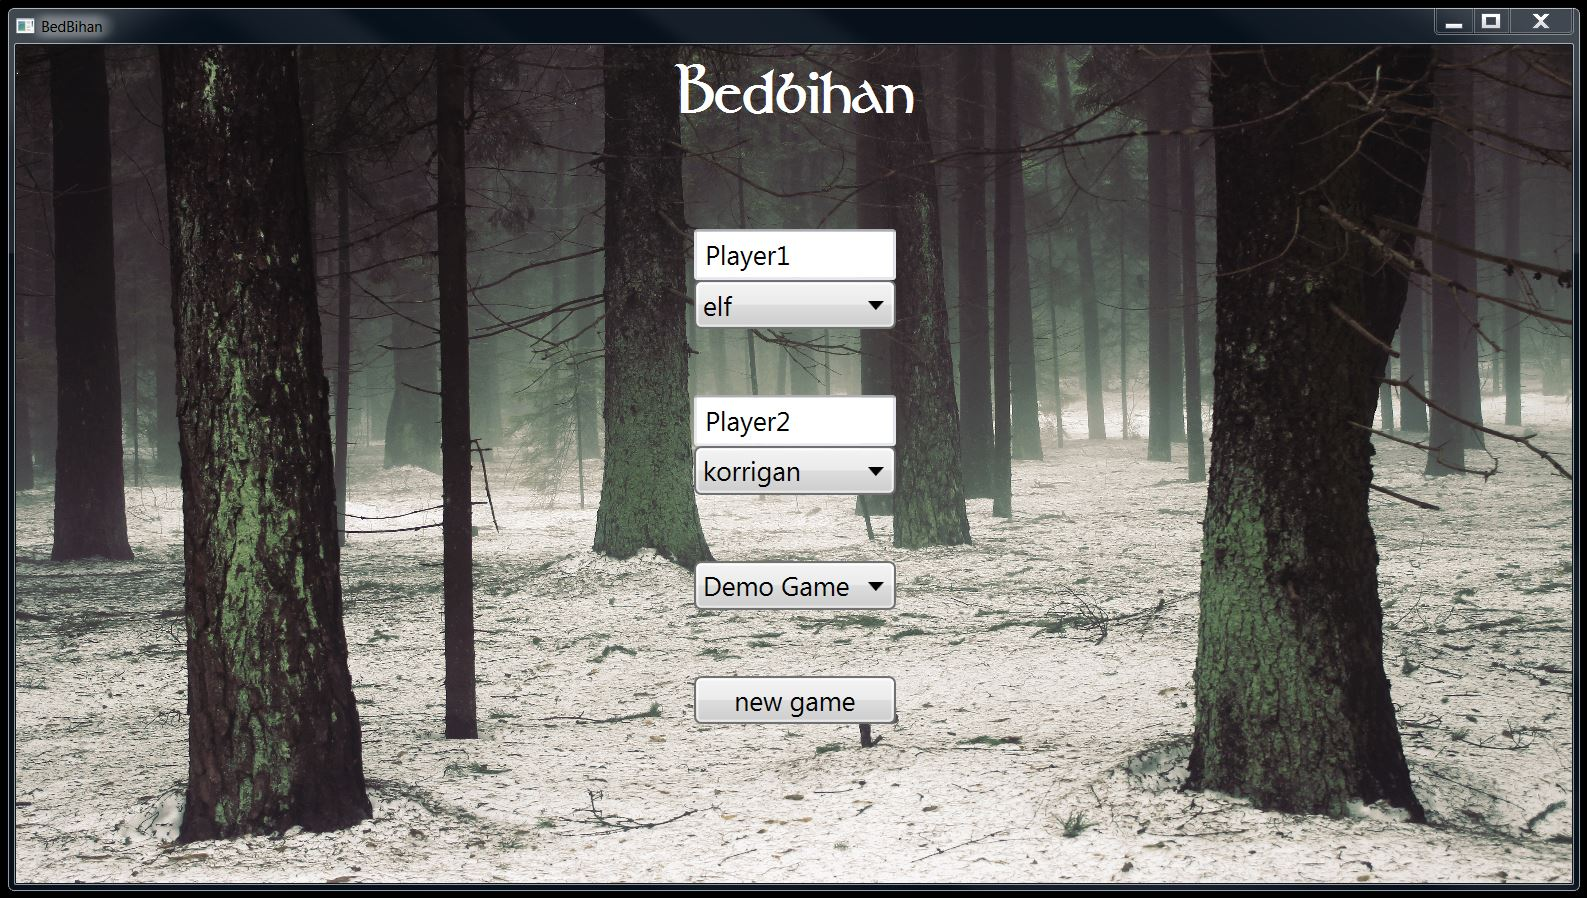
\includegraphics[width=0.9\textwidth]{figure/mainmenu.png}
			\end{center}
			\caption{Menu principal permettant de créer une nouvelle partie.}
			\label{fig:launch}
		\end{figure}

		\subsection{Sélection d'une unité}
		Chaque joueur, lorsque c'est son tour, peut cliquer sur les cases de la carte en utilisant le {\bf clic-gauche de la souris} pour connaitre les unités actuellement situées sur cette case. Les unités s'affichent à gauche, et par défaut la première unité de la liste est sélectionnée, comme indiqué sur la {\sc Figure }{\ref {fig:usco}}. 
		
		\begin{figure}
			\begin{center}
				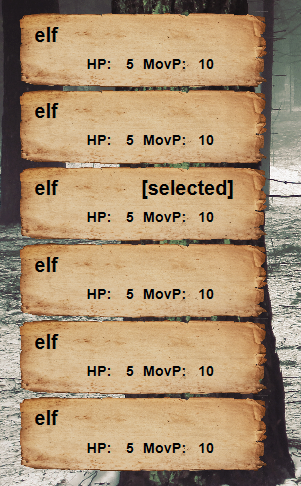
\includegraphics[width=0.4\textwidth]{figure/unitscore.png}
			\end{center}
			\caption{Liste des unités présentes sur une case.}
			\label{fig:usco}
		\end{figure}
		
		
		Le joueur peut cliquer sur une autre unité de cette liste pour la sélectionner, en utilisant le {\bf clic-gauche de la souris}. Dans le panneau latéral de droite, comme indiqué sur la {\sc Figure }{\ref {fig:stat}}, les statistiques de l'unité sélectionnées s'affichent : points de vie, attaque, défense, etc. sont indiqués en détails.		
		
		\begin{figure}
			\begin{center}
				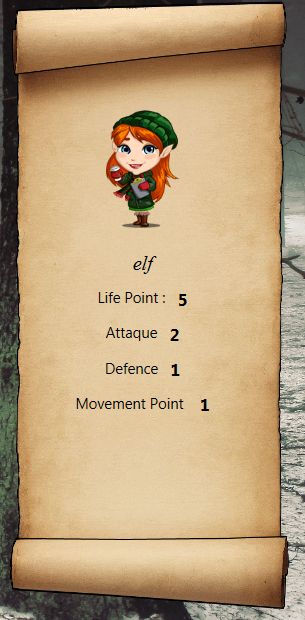
\includegraphics[width=0.3\textwidth]{figure/stats.png}
			\end{center}
			\caption{Statistiques d'une unité.}
			\label{fig:stat}
		\end{figure}
		
		\newpage
		\subsection{Déplacement d'une unité}
		Si l'unité sélectionnées est une unité appartenant au joueur, les cases sur lesquelles il peut la déplacer voient leur contour s'afficher en vert, comme indiqué sur la {\sc Figure }{\ref {fig:case}}. Pour bouger une unité, le joueur doit cliquer sur l'une des cases dont le contour est en vert en utilisant le {\bf clic-droit de la souris}.
		
		\begin{figure}[h!]
			\begin{center}
				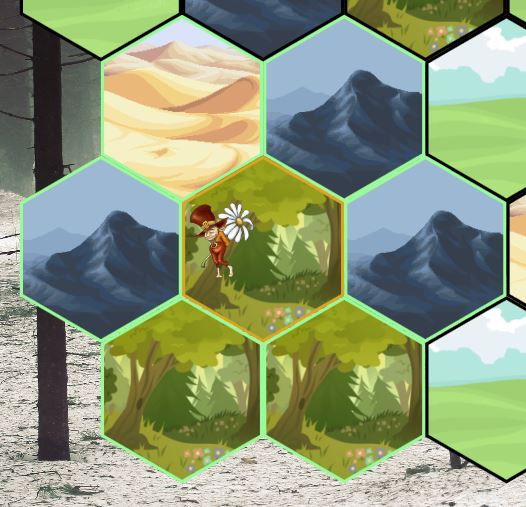
\includegraphics[width=0.6\textwidth]{figure/caseaccessible.jpg}
			\end{center}
			\caption{Cases aux bordures vertes indiquant que l'unité sélectionnée peut s'y déplacer.}
			\label{fig:case}
		\end{figure}
		
		\paragraph{Remarque} Le clic-gauche sert à sélectionner une case pour avoir des informations. Faites donc bien attention à utiliser le {\bf clic-droit} pour déplacer une unité sur une case accessible.
		
		
		\subsection{Combat entre unités}
		Pour se battre contre une unité adverse située sur une case donnée, il est nécessaire que cette case soit accessible par l'unité sélectionnée. Si cette condition est remplie, il suffit de tenter de se déplacer sur cette case occupée en utilisant le {\bf clic-gauche de la souris}. Un combat a alors lieu automatiquement contre l'unité la plus résistante de cette case. L'issue de ce combat est affichée dans une boite de dialogue telle qu'indiquée sur la {\sc Figure }{\ref {fig:comb}}.
		
		\begin{figure}
			\begin{center}
				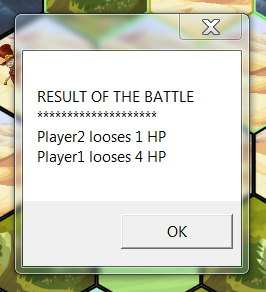
\includegraphics[width=0.3\textwidth]{figure/issuecomb.png}
			\end{center}
			\caption{Issue possible d'un combat.}
			\label{fig:comb}
		\end{figure}
		
		
		\subsection{Fin du tour}
		Lorsqu'un joueur estime qu'il a terminé son tour, il peut cliquer sur le bouton \og End turn \og{} situé en bas de la fenêtre, comme indiqué sur la {\sc Figure }{\ref {fig:endturn}}. Une petite animation indique alors que c'est au joueur suivant de jouer son tour.
		
		\begin{figure}
			\begin{center}
				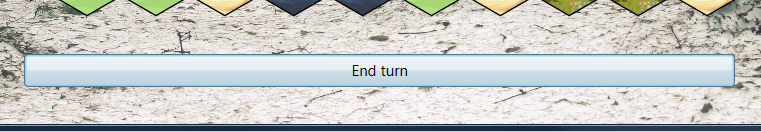
\includegraphics[width=0.8\textwidth]{figure/endturn.png}
			\end{center}
			\caption{Bouton permettant de terminer le tour actuel.}
			\label{fig:endturn}
		\end{figure}
		
		Le nom du joueur dont c'est le tour, le nombre de tour maximum ainsi que le numéro du tour courant sont affiché en haut à droite de la fenêtre, comme indiqué sur la {\sc Figure }{\ref {fig:turn}}.
		
		\begin{figure}
			\begin{center}
				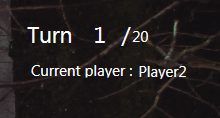
\includegraphics[width=0.4\textwidth]{figure/turn.png}
			\end{center}
			\caption{Informations sur le tour actuel de la partie.}
			\label{fig:turn}
		\end{figure}
				
		
		
		
		\subsection{Points}
		Les points sont calculés à la fin du tour de chaque joueur. Le score est affiché en haut à gauche de la fenêtre, comme indiqué sur la {\sc Figure }{\ref {fig:score}}.
		
		\begin{figure}
			\begin{center}
				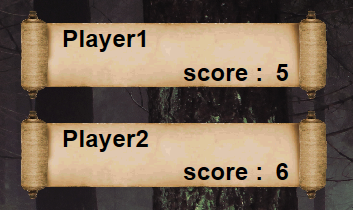
\includegraphics[width=0.4\textwidth]{figure/score.png}
			\end{center}
			\caption{Score actuel des joueurs.}
			\label{fig:score}
		\end{figure}
		
		\subsection{Fin de la partie}
		La partie se termine lorsqu'un joueur a perdu toutes ses unités, ou que le nombre de tours impartis est écoulé. Le vainqueur de la partie est alors affiché dans une boite de dialogue, comme indiqué sur la {\sc Figure }{\ref {fig:end}}.
		
		\begin{figure}
			\begin{center}
				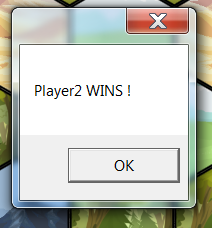
\includegraphics[width=0.3\textwidth]{figure/winner.png}
			\end{center}
			\caption{Vainqueur de la partie.}
			\label{fig:end}
		\end{figure}
		
		Un joueur peut également terminer la partie en cliquant sur le bouton \og Exit game \fg{} situé tout en haut à gauche de la fenêtre, comme indiqué sur la {\sc Figure }{\ref {fig:exit}}.
		
		\begin{figure}
			\begin{center}
				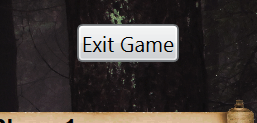
\includegraphics[width=0.5\textwidth]{figure/exit.png}
			\end{center}
			\caption{Bouton permettant de quitter la partie.}
			\label{fig:exit}
		\end{figure}